% Part 3, chapter on the background quasiparticle density in Al/AlOx/Al transmons.
% Numbers: docs/verification/scripts/verify_xqp_book.py (+ _output.txt); earlier check script verify_xqp.py.
% Corrections: docs/verification/PAPER_ERRATA.md rows XQ1-XQ8; docs/verification/particle/XQP_CHECK.md, XQP_REFEREE_NOTE.md;
% source checks of this carriage: docs/book/read_ledgers/MANIFEST_xqp.md. Figures: figscripts/fig_p3.py (thermal, sites),
% figscripts/fig_p3_xqp_book.py (ladder, london, tau). Bibliography additions: bib_xqp.bib.
\chapter{The cost of holding a qubit}\label{ch:xqp}

\section*{The place}
IAM's Law (Chapter~\ref{ch:iams_law}) prices every irreversible record at $\kB T\ln2$ per bit at the nearest encoding surface
(Eq.~\eqref{eq:law_landauer}). A superconducting qubit is a device built to \emph{avoid} records: it holds a superposition for as long as it
can. This chapter asks what the law says that holding costs, and where the cost should appear in a measurement. The proposal is that part of the
background density of broken Cooper pairs in Al/AlO$_x$/Al transmons is endogenous: the thermodynamic cost of maintaining quantum coherence
against the bath of two-level fluctuators (TLS) in the oxide barrier, paid continuously at the junction whether or not the qubit is being used
\conjecture. The chapter states the anomaly, the proposal and its three assumptions, derives each step from superconductor physics, gives the
steady-state density in the units in which the floor is measured, and ends with a test that one device can pass or fail.

\section{The anomaly}\label{sec:xqp_anomaly}

\begin{figure}[htbp]\centering
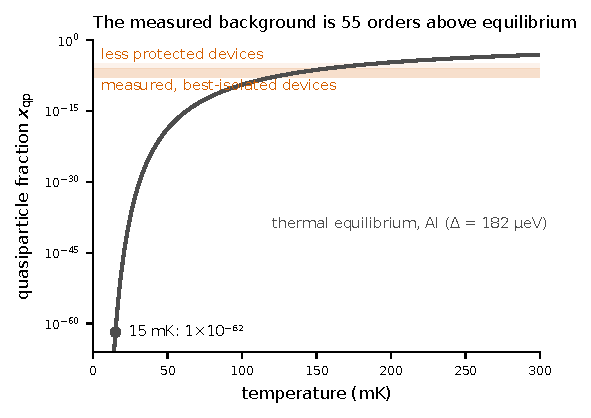
\includegraphics[width=0.62\textwidth]{figures/part3/fig_xqp_thermal.pdf}
\caption{Equilibrium quasiparticle fraction in aluminium, $x_{\rm qp}=\sqrt{2\pi k_BT/\Delta}\,e^{-\Delta/k_BT}$ with $\Delta=182\,\mu$eV \calc: $1.5\times10^{-62}$ at 15\,mK ($\Delta/k_BT=141$), reaching $10^{-7}$ only near 135\,mK. Shaded: the background commonly measured in transmons, $10^{-8}$--$10^{-6}$, and up to $10^{-5}$ in less protected devices \observed; the best reported device reaches $\lesssim10^{-9}$ (text).}\label{fig:xqp_thermal}
\end{figure}
Non-equilibrium quasiparticles are broken Cooper pairs. They limit the coherence of superconducting qubits by tunnelling across the Josephson
junction. In Al/AlO$_x$/Al transmons the measured density of quasiparticles is commonly
\begin{equation}x_{\rm qp}=n_{\rm qp}/n_{\rm cp}\sim10^{-8}\text{--}10^{-6},\qquad n_{\rm cp}=2\nu_0\Delta\approx4\times10^6\,\mu{\rm m}^{-3},\label{eq:xqp_def}\end{equation}
with $x_{\rm qp}\approx10^{-7}$ in many devices~\cite{Serniak2018,Diamond2022PRXQ}, that is $n_{\rm qp}\approx0.4$ per $\mu$m$^3$ \observed. Here $\nu_0$ is
the single-spin density of states at the Fermi level, and $n_{\rm cp}=2\nu_0\Delta$ counts the electrons within about $\Delta$ of the Fermi surface,
the states that the gap actually rearranges~\cite{Riste2013,Wang2014,Glazman2021}. With $\nu_0=1.2\times10^4\,\mu$m$^{-3}\,\mu$eV$^{-1}$ for Al~\cite{Riste2013}
it is $4.1$--$4.4\times10^6\,\mu$m$^{-3}$ for $\Delta=170$--$182\,\mu$eV; the free-electron density of states of Al gives $4.2\times10^6\,\mu$m$^{-3}$
\calc. The lowest reported value is $x_{\rm qp}\lesssim10^{-9}$~\cite{Connolly2024}; the density $n_{\rm qp}=0.04\,\mu$m$^{-3}$ reported at 20\,mK
in Ref.~\cite{Riste2013} is $x_{\rm qp}\approx1\times10^{-8}$ \calc. In thermal equilibrium at 15--20\,mK there should be fewer than one
quasiparticle in a volume the size of the Earth \calc. The floor has persisted for two decades of measurements while the known external sources
have been reduced one by one: stray infrared light~\cite{Barends2011}, environmental radioactivity~\cite{Vepsalainen2020,Cardani2021} and cosmic
rays~\cite{McEwen2022}. An excess over equilibrium remains. What the measurements show, read carefully:
\begin{itemize}
\item \emph{Underground.} The same transmon was measured above ground at Fermilab and deep underground at Gran Sasso, where the 1.4\,km rock
overburden reduces muon interactions by six orders of magnitude and copper and lead shields reduce the gamma background. It shows a
similar average $T_1$ of about 80\,$\mu$s at both sites~\cite{DeDominicis2026}; the same study still found a significant excess of
radiation-induced events above ground. $T_1$ is insensitive to added shielding while the quasiparticle tunnelling rate is very sensitive to
it~\cite{Gordon2022}. Together these say that at present lifetimes $T_1$ is not set by radiation-generated quasiparticles, and that a large part of
the measured tunnelling is of external origin. They do not by themselves show an internal source \observed.
\item \emph{Energy distribution.} The excess quasiparticles have an energy distribution in equilibrium with the phonon bath, coexisting with a density
far above equilibrium~\cite{Connolly2024}. External sources deposit quasiparticles above the gap; in aluminium they relax to the gap edge by phonon
emission far faster than they recombine at these densities~\cite{Kaplan1976}, so any source gives this distribution. It is consistent with a
continuous internal source but does not single one out \observed.
\item \emph{Junction and capacitor.} The tunnelling rate of the non-equilibrium quasiparticles depends on the shunting-capacitor material and
geometry, and in some designs scales with the capacitor area~\cite{Kurter2022}. In some devices an anomalous temperature dependence below
100\,mK departs from the flat non-equilibrium background; it has been modelled as high-transmission sites in the junction barrier with a smaller
effective gap $\Delta_1$, design medians 5--30\,$\mu$eV against bulk medians $\Delta_0=183$--$193\,\mu$eV~\cite{Kurter2022} \observed.
\item \emph{Correlations.} Individual background tunnelling events are uncorrelated between two co-housed qubits, while bursts, about once per minute,
are correlated across devices~\cite{Sundelin2026,McEwen2022} \observed.
\item \emph{Where the fluctuators are.} Most detectable surface TLS sit on the leads of the Josephson junction, not on the capacitor that dominates
the field energy and surface area~\cite{Lisenfeld2025}; quasiparticles trapped in gap inhomogeneities can themselves act as TLS~\cite{deGraaf2020}
\observed.
\end{itemize}
These leave room for a source inside the device, at the junction; they do not establish it. The proposal below is that source, stated so that a
measurement can rule it in or out.

\section{The proposal}\label{sec:xqp_proposal}
\conjecture\ Three assumptions carry the proposal, each stated here and developed from superconductor theory in
Section~\ref{sec:xqp_foundations}: (i) maintaining coherence against the TLS bath is a Landauer erasure; (ii) the erasure is charged at the gap
scale $T_{\rm gap}=\Delta_{\rm Al}/\kB$; (iii) each erasure involves the condensate within a London depth of its site. A fourth fact, not an
assumption, turns events into a density: the quasiparticles created spread over the whole island (Section~\ref{sec:xqp_events}).

\paragraph{The encoding surface and the maintenance cost.} The Al/AlO$_x$/Al junction holds a quantum superposition against continuous
decoherence pressure from the TLS bath in the AlO$_x$ barrier and at the metal--oxide interfaces~\cite{Phillips1987,Muller2019}. It does not
perform this maintenance only when a decoherence event occurs; it holds coherence continuously, restoring its state at the rate set by the
fluctuations it must resist. A control system that re-executes its state estimate at fixed intervals, whether or not conditions have changed, is
the analogy: the cost is structural, not conditional \interp.

\paragraph{The rate.} The time scale is $\tTLS$, the switching time of the fluctuators that produce the $1/f$ charge and frequency noise of the
barrier. Long-time measurements on superconducting resonators show $1/f$ noise down to 0.1\,Hz that grows at low temperature, the signature of
interacting TLS whose switching times are spread over many decades~\cite{Burnett2014}; individual TLS switch on microseconds to hours
(Chapter~\ref{ch:scprimer}) \observed. The fluctuators that matter here are the active ones near the junction. This chapter uses
$\tTLS=30\,\mu$s as a working value inside a 1--100\,$\mu$s working range; a device has to supply its own value, measured from its $1/f$ noise.

\paragraph{The irreversibility.} A TLS flip kicks the condensate phase at the site. The condensate restores its phase in $\hbar/\Delta\approx3.6$\,ps,
five to seven orders of magnitude faster than the next flip. After restoration the condensate is the same whichever way the TLS flipped: the
information about the flip has been discarded. That is an erasure in the sense of Landauer and Bennett~\cite{Landauer1961,Bennett1982}, and by
IAM's Law it is paid in heat, at least $\kB T_H\ln2$ to a bath at temperature $T_H$. Each active site therefore produces an irreversible event at
rate $1/\tTLS$, whether or not the qubit is being used. The separation of time scales makes the events independent, as the uncorrelated
background events require \conjecture.

\paragraph{Which temperature.} In conventional thermodynamics the Landauer cost of resetting a degree of freedom is paid to the reservoir that
absorbs the heat, here the phonons at $\sim20$\,mK, where $\kB T\ln2$ is about $1.2\,\mu$eV \calc. Charging the erasure at the condensate's own
scale, $T_{\rm gap}=\Delta_{\rm Al}/\kB=2.11$\,K, is IAM's Law applied to the nearest encoding surface \conjecture. It is the one place in this
chapter where IAM departs from standard thermodynamics, and therefore the place a clean experiment decides. $T_{\rm gap}$ is an energy scale written
as a temperature: aluminium is normal above $T_c=1.20$\,K, so no part of the film is at 2.11\,K \calc.

\paragraph{The scales.} The junction sits within a hierarchy of scales (Figure~\ref{fig:xqp_ladder}):
\begin{equation}T_{\rm CMB}=2.725\ {\rm K}\;>\;T_{\rm gap}=\Delta_{\rm Al}/\kB=2.11\ {\rm K}\;>\;T_c=1.20\ {\rm K}\;\gg\;T_{\rm fridge}\approx15\ {\rm mK}.\label{eq:xqp_ladder}\end{equation}
The gaps are $T_{\rm CMB}-T_{\rm gap}=0.61$\,K and $T_{\rm gap}-T_{\rm fridge}=2.10$\,K \calc. The cosmic microwave background is the ambient
radiation of the universe; inside a cryostat it never reaches the chip, which sees only the warmer shields and wiring
(Chapter~\ref{ch:scprimer}).

\begin{figure}[htbp]\centering
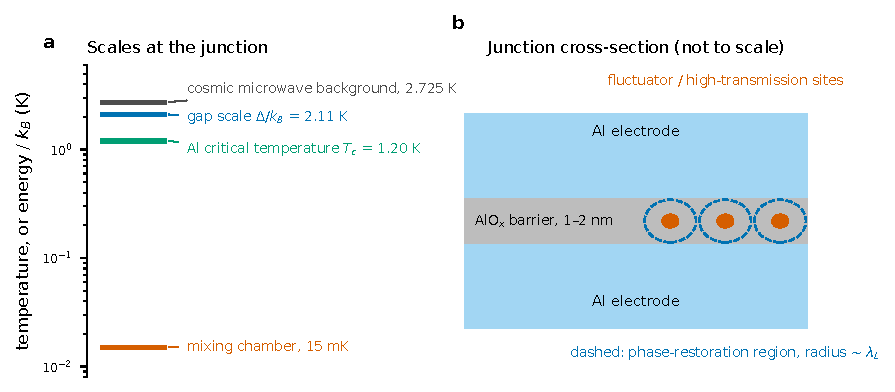
\includegraphics[width=\textwidth]{figures/part3/fig_xqp_ladder.pdf}
\caption{(a) Scales at an Al/AlO$_x$/Al junction written as temperatures, Eq.~\eqref{eq:xqp_ladder}: the cosmic microwave background, the gap scale
$\Delta_{\rm Al}/k_B=2.11$\,K at which the proposal charges each erasure, the critical temperature of aluminium and the mixing chamber \calc. (b) The
junction cross-section: a 1--2\,nm AlO$_x$ barrier between Al electrodes, with fluctuator and high-transmission sites in and at the barrier
\observed; dashed, the region within about $\lambda_L$ that takes part in each phase restoration, Eq.~\eqref{eq:xqp_veff} \conjecture.}\label{fig:xqp_ladder}
\end{figure}

\section{Theoretical foundations}\label{sec:xqp_foundations}
Each assumption is now developed from the London equations, the BCS density of states and the Landauer--Bennett bound. The derivations make the
assumptions precise; they do not make them established. Which parts survive contact with the physics of pair breaking and diffusion is the subject
of Section~\ref{sec:xqp_events}.

\subsection{The phase-disturbance volume from the London equation}\label{sec:xqp_london}
A tunnelling or fluctuator event at a site creates a localized phase disturbance in the Al condensate. Its spatial extent follows from the London
equation. In the Coulomb gauge the vector potential in the bulk superconductor obeys
\begin{equation}\nabla^2\mathbf A=\frac{\mathbf A}{\lambda_L^2}.\label{eq:xqp_london}\end{equation}
A point-like current perturbation at the site ($r=0$) acts as a localized source. The Green's function of
$(\nabla^2-\lambda_L^{-2})G=-\delta^3(\mathbf r)$ gives
\begin{equation}\mathbf A(r)=\frac{\mu_0\mathbf J_{\rm pin}}{4\pi}\,\frac{e^{-r/\lambda_L}}{r}.\label{eq:xqp_green}\end{equation}
\derived\ (for $r>0$, $(\nabla^2-\lambda_L^{-2})\,e^{-r/\lambda_L}/(4\pi r)=0$; checked symbolically). The condensate phase gradient couples to
$\mathbf A$ through the London relation $\nabla\phi=(2e/\hbar)\mathbf A$, so the phase disturbance falls off as $\delta\phi(r)\sim e^{-r/\lambda_L}$
for $r\gg0$.

Define the participation volume as the phase-weighted integral of the disturbance, with the exponential envelope normalised to its value at the
site:
\begin{equation}V_{\rm eff}=\int\left|\frac{\delta\phi(r)}{\delta\phi(0)}\right|^2d^3r=4\pi\int_0^\infty e^{-2r/\lambda_L}\,r^2\,dr.\label{eq:xqp_veff_int}\end{equation}
With $u=2r/\lambda_L$,
\begin{equation}V_{\rm eff}=4\pi\,\frac{\lambda_L^3}{8}\int_0^\infty u^2e^{-u}\,du=4\pi\,\frac{\lambda_L^3}{8}\,\Gamma(3)=\pi\lambda_L^3.\label{eq:xqp_veff}\end{equation}
\derived\ The integral is exact and is fixed by the London screening length alone; for $\lambda_L=50$\,nm (Al films~\cite{Kurter2022,Greytak1964}) it is
$3.93\times10^{-22}$\,m$^3=3.9\times10^{-4}\,\mu$m$^3$ \calc\ (Figure~\ref{fig:xqp_london}). Two assumptions sit inside it, and both are stated:
the weight is the square of the phase disturbance, and the $1/r$ factor of Eq.~\eqref{eq:xqp_green} is absorbed into the normalisation. Keeping the
full profile $e^{-r/\lambda_L}/r$ and normalising it at a core radius $r_0$ gives $2\pi\lambda_L r_0^2$ instead, which depends on the core
\calc.

The scale is $\lambda_L$, not the BCS coherence length $\xi_0\approx1.6\,\mu$m of bulk Al~\cite{Kittel2005}. The two describe different physics:
$\xi_0$ is the amplitude coherence length, over which $|\Delta(\mathbf r)|$ recovers after pair breaking; $\lambda_L$ is the phase screening length,
which governs how far a phase disturbance of the superfluid extends. The erasure discards phase information, not pairs, so $\lambda_L$ is the scale
for the restoration \interp. Using $\xi_0$ would give a volume $(\xi_0/\lambda_L)^3=(1600/50)^3\approx3\times10^4$ times larger \calc. In Al the two
lengths are cleanly separated: $\lambda_L/\xi_0\approx0.03\ll1$, a type-I superconductor in bulk \calc.

\paragraph{What the volume is, and what it is not.} $\pi\lambda_L^3$ is the volume of condensate that takes part in one phase restoration at one
site. It is \emph{not} the volume that holds the quasiparticles afterwards: those diffuse across the island within their lifetime
(Section~\ref{sec:xqp_events}). The volume therefore does not enter the measured density.

\begin{figure}[htbp]\centering
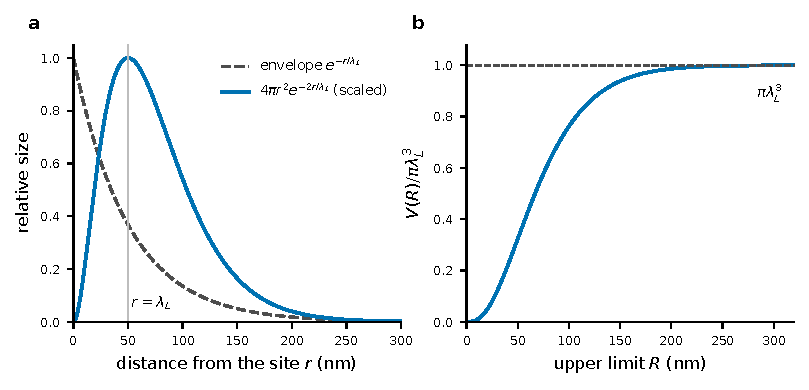
\includegraphics[width=\textwidth]{figures/part3/fig_xqp_london.pdf}
\caption{The London participation volume, Eqs.~\eqref{eq:xqp_veff_int}--\eqref{eq:xqp_veff}, for $\lambda_L=50$\,nm. (a) The phase envelope
$e^{-r/\lambda_L}$ and the integrand $4\pi r^2e^{-2r/\lambda_L}$, which peaks at $r=\lambda_L$. (b) The running integral reaches $\pi\lambda_L^3$
(99.998\,\% by $R=400$\,nm). \derived}\label{fig:xqp_london}
\end{figure}

\subsection{The gap scale as the bath of the erasure}\label{sec:xqp_bath}
Landauer's principle needs the temperature of the bath that receives the erasure energy. The proposal takes it from the BCS density of states. The
condensate at a site can exchange energy only with excitations above the gap, whose density of states is
\begin{equation}N(E)=N_0\,\frac{E}{\sqrt{E^2-\Delta_{\rm Al}^2}},\qquad E>\Delta_{\rm Al},\label{eq:xqp_bcsdos}\end{equation}
with $N(E)=0$ for $E<\Delta_{\rm Al}$. Counting both spins and both branches, the equilibrium quasiparticle density at $\kB T\ll\Delta$ is
$n_{\rm qp}=4\nu_0\int_\Delta^\infty \frac{E}{\sqrt{E^2-\Delta^2}}\,e^{-E/\kB T}\,dE=4\nu_0\Delta\,K_1(\Delta/\kB T)$, and with
$K_1(z)\simeq\sqrt{\pi/2z}\,e^{-z}$ for $z\gg1$ the thermal fraction is
\begin{equation}x_{\rm qp}^{\rm th}(T)=\frac{n_{\rm qp}}{2\nu_0\Delta}\simeq\sqrt{\frac{2\pi\kB T}{\Delta_{\rm Al}}}\;e^{-\Delta_{\rm Al}/\kB T},\qquad \kB T\ll\Delta_{\rm Al}.\label{eq:xqp_xth}\end{equation}
\derived\ (sympy, and the exact $2K_1$ form agrees to 0.4\,\% at 20\,mK and 3\,\% at 150\,mK). Two candidate baths exist at the site.

\emph{Bath A, substrate phonons at $T_{\rm fridge}$.} At 15\,mK the Boltzmann factor for a quasiparticle excitation is
$e^{-\Delta_{\rm Al}/\kB T_{\rm fridge}}=e^{-141}\approx10^{-61}$ \calc. The phonon bath cannot break pairs at this temperature; for
quasiparticle-generating processes it is effectively decoupled from the condensate.

\emph{Bath B, the quasiparticle continuum above the gap.} The scale at which the quasiparticle bath becomes thermally accessible is
$\kB T_{\rm eff}\sim\Delta_{\rm Al}$:
\begin{equation}T_{\rm gap}\equiv\frac{\Delta_{\rm Al}}{\kB}=2.11\ {\rm K}.\label{eq:xqp_tgap}\end{equation}
At this scale the thermal fraction of Eq.~\eqref{eq:xqp_xth} is of order unity (the low-temperature form, used beyond its range, gives 0.92)
\calc. The argument for Bath B is that an erasure which produces quasiparticles delivers its energy to the quasiparticle continuum; the temperature
in the Landauer bound is then that continuum's scale, fixed by the material gap with no free parameter. Any lower temperature would leave
quasiparticle-generating erasure thermally inaccessible; any higher one would imply a different gap \conjecture. This is the assumption (ii)
of Section~\ref{sec:xqp_proposal}, and it is a conjecture of IAM, not a result of BCS theory: in standard thermodynamics the erasure heat flows to
whatever reservoir finally absorbs it.

\paragraph{The refrigerator temperature.} The assignment implies that the floor should not follow $T_{\rm fridge}$ while
$T_{\rm fridge}\ll T_{\rm gap}$ \prediction. Ref.~\cite{Riste2013} found the parity-switching rates rising with refrigerator temperature over
20--170\,mK, with a suppression at low temperature much weaker than a thermal distribution predicts, and $T_1$ insensitive to temperature up to
150\,mK \observed. A floor that stops following $T_{\rm fridge}$ at the lowest temperatures is what any non-thermal source gives, so this
observation is consistent with the gap-scale assignment but does not discriminate it from generated-quasiparticle models.

\subsection{The erasure mapping}\label{sec:xqp_mapping}
TLS-induced decoherence of the condensate phase at a site is now cast as a Landauer erasure in the sense of Bennett~\cite{Bennett1982}. Consider
the joint state of the condensate phase $\phi$ and one TLS at the site. The TLS couples to the phase through the junction admittance with strength
$g$. Measured TLS--qubit couplings in Al/AlO$_x$/Al junctions are $g/2\pi\sim1$--10\,MHz~\cite{Lisenfeld2019,deGraaf2020}, against qubit frequencies
$\omega_q/2\pi\sim5$\,GHz. A single TLS flip $|s\rangle\to|s'\rangle$ imprints a phase kick of order
\begin{equation}\delta\phi\sim\frac{g}{\omega_q}\sim2\times10^{-4}\text{--}2\times10^{-3}\ {\rm rad}.\label{eq:xqp_kick}\end{equation}
\calc\ This is small against $2\pi$, so the system is perturbative. The value of $\delta\phi$ does not enter the energy bound: the minimum
erasure cost holds for any nonzero kick, provided the restoration is irreversible. The condition $\delta\phi\ll1$ is needed only to treat each flip
as an independent event, which the separation of time scales confirms on its own. The condensate restores its phase by dissipative relaxation on
\begin{equation}\tau_\phi\sim\frac{\hbar}{\Delta_{\rm Al}}=3.6\ {\rm ps},\label{eq:xqp_tauphi}\end{equation}
faster than the TLS switching time by
\begin{equation}\frac{\tau_\phi}{\tTLS}\sim\frac{\hbar/\Delta_{\rm Al}}{\tTLS}=\frac{3.6\ {\rm ps}}{30\ \mu{\rm s}}=1.2\times10^{-7}\label{eq:xqp_sep}\end{equation}
\calc\ ($3.6\times10^{-6}$ to $3.6\times10^{-8}$ over 1--100\,$\mu$s; Chapter~\ref{ch:scprimer}, Figure~\ref{fig:timescales}). The separation has two
consequences. Each flip is a complete erasure before the next flip occurs, and the events are statistically independent, consistent with the
uncorrelated background tunnelling events of Ref.~\cite{Sundelin2026}. In the language of open quantum systems, $\tau_\phi\ll\tTLS$ is the Markovian
limit: the condensate's memory of each perturbation decays far faster than the interval between events, so each flip is an independent quantum
jump whose minimum dissipation is set by the Landauer--Bennett bound \interp.

The logical irreversibility is this. After a flip the condensate phase carries information about which TLS state caused the perturbation,
$|s\rangle$ or $|s'\rangle$. The restoration $\phi_0+\delta\phi\to\phi_0$ discards it: the restored condensate is identical whichever way the TLS
flipped. Discarding one bit about the TLS state is a Landauer erasure~\cite{Landauer1961,Bennett1982}. With the bath at the gap scale the minimum
heat is
\begin{equation}E_{\rm erase}=\kB T_{\rm gap}\ln2=\frac{\Delta_{\rm Al}}{\kB}\,\kB\ln2=\Delta_{\rm Al}\ln2=126\ \mu{\rm eV}.\label{eq:xqp_erase}\end{equation}
\conjecture\ (given assumption (ii); the arithmetic is exact). The identification $T_H=T_{\rm gap}$ is what enters here: the bath temperature in the
bound is that of the quasiparticle continuum. Equation~\eqref{eq:xqp_erase} is a minimum heat. It is not a number of quasiparticles; the next section
fixes the yield.

\section{From events to quasiparticles}\label{sec:xqp_events}
Three facts of superconductor physics fix how events become a density.
\paragraph{Pair breaking is quantised.} A quasiparticle exists only once a Cooper pair is broken, which costs $2\Delta$ ($364\,\mu$eV in Al) and yields
two quasiparticles. Landauer's principle sets the \emph{minimum} heat of an erasure~\cite{Landauer1961}, $\Delta\ln2=126\,\mu$eV if the bath sits at the
gap scale; heat released below $2\Delta$ goes into sub-gap phonons that cannot break pairs. An erasure event that produces quasiparticles therefore
breaks a pair: yield $Y=2$ per event. If only a fraction $p$ of events break a pair, the yield is $Y=2p$.
\paragraph{Quasiparticles spread.} In aluminium they diffuse $\sqrt{D\tau_{\rm qp}}\approx250$--$800\,\mu$m within a lifetime $\tau_{\rm qp}\sim100\,\mu$s
($D\approx0.6$--$6\,\mu$m$^2$/ns) \calc, across the whole island; models of quasiparticle poisoning treat the electrodes as having a uniform
density~\cite{Yelton2024}. What a qubit measures is the island average, not the density inside $\pi\lambda_L^3$.
\paragraph{The density is per pair near the gap.} $n_{\rm cp}=2\nu_0\Delta$ counts the electrons within $\Delta$ of the Fermi surface, not all
conduction electrons ($n_e/2=9.03\times10^{10}\,\mu$m$^{-3}$ for three electrons per atom on an FCC lattice with $a=4.05$\,\AA, which is $22{,}600$
times larger) \calc.

\paragraph{The steady state.} Let $N$ active sites on an island of volume $V$ each produce events at rate $1/\tTLS$ with yield $Y$, and let
quasiparticles disappear with lifetime $\tqp$. The number $N_{\rm qp}$ on the island obeys
\begin{equation}\frac{dN_{\rm qp}}{dt}=\frac{YN}{\tTLS}-\frac{N_{\rm qp}}{\tqp},\qquad N_{\rm qp}(t)=\frac{YN\tqp}{\tTLS}\left(1-e^{-t/\tqp}\right),\label{eq:xqp_rate}\end{equation}
so the steady state is $N_{\rm qp}=YN\tqp/\tTLS$. Dividing by $n_{\rm cp}V$ and setting $Y=2$,
\begin{equation}x_{\rm qp}=\frac{2N\,\tau_{\rm qp}}{\tau_{\rm TLS}\,n_{\rm cp}\,V}.\label{eq:xqp}\end{equation}
\derived\ (from the proposal and the three facts above; sympy). The generation rate per site is $\Gamma_{\rm qp}=Y/\tTLS$ quasiparticles per
second, and the minimum heat it carries is $2\Delta/\tTLS=1.9\times10^{-18}$\,W per site, $1.2\times10^{-15}$\,W for 600 sites \calc, far
below the cooling power of a mixing chamber.

\paragraph{Inputs.} Table~\ref{tab:xqp_inputs} lists the values used for the numbers below; each is a material value or a working value, and on a
real device each is measured.
\begin{table}[htbp]\centering
\caption{Inputs to Eq.~\eqref{eq:xqp}.}\label{tab:xqp_inputs}
\begin{tabular}{p{3.3cm}p{3.5cm}p{7.6cm}}\toprule
quantity & value & source and status\\\midrule
gap $\Delta_{\rm Al}$ & $182\,\mu$eV ($T_{\rm gap}=2.112$\,K) & BCS $1.764\,\kB T_c$ at $T_c=1.20$\,K \calc; design medians 183--193\,$\mu$eV~\cite{Kurter2022} \observed\\
Cooper-pair density $n_{\rm cp}$ & $4\times10^6\,\mu$m$^{-3}$ & $2\nu_0\Delta$, Eq.~\eqref{eq:xqp_def}~\cite{Riste2013,Wang2014} \calc\\
TLS switching time $\tTLS$ & $30\,\mu$s (range 1--100\,$\mu$s) & working value; measured per device from $1/f$ noise~\cite{Burnett2014}\\
quasiparticle lifetime $\tqp$ & $100\,\mu$s & working value; measured per device~\cite{Lenander2011,Wang2014}\\
London depth $\lambda_L$ & 50\,nm & Al films~\cite{Kurter2022,Greytak1964} \observed; enters $V_{\rm eff}$ only\\
active sites $N$ & to be measured & TLS spectroscopy~\cite{Lisenfeld2019,Lisenfeld2025}\\
island volume $V$ & $10^3$--$10^5\,\mu$m$^3$ & device geometry\\\bottomrule
\end{tabular}
\end{table}

\section{What it requires}\label{sec:xqp_requires}

\begin{figure}[htbp]\centering
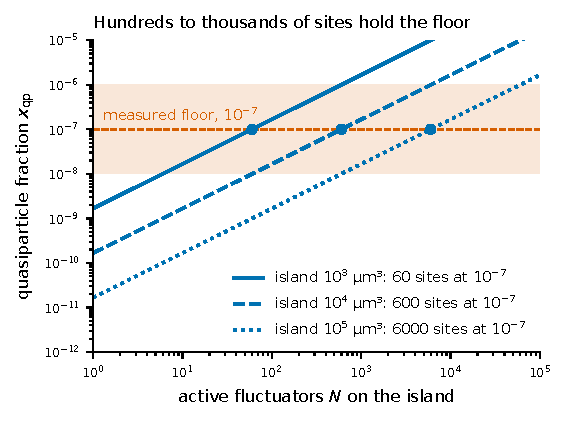
\includegraphics[width=0.62\textwidth]{figures/part3/fig_xqp_sites.pdf}
\caption{Eq.~\eqref{eq:xqp} with yield 2 per event, $n_{\rm cp}=4\times10^{6}\,\mu$m$^{-3}$, $\tau_{\rm TLS}=30\,\mu$s and $\tau_{\rm qp}=100\,\mu$s, for islands of $10^3$, $10^4$ and $10^5\,\mu$m$^3$: 60, 600 and 6,000 active fluctuators hold $10^{-7}$ (band: $10^{-8}$--$10^{-6}$). \derived\ (form) \calc\ (values)}\label{fig:xqp_sites}
\end{figure}
\begin{table}[htbp]\centering
\caption{Active sites needed for the measured floor, Eq.~\eqref{eq:xqp} with $\tTLS=30\,\mu$s and $\tqp=100\,\mu$s. \calc}\label{tab:xqp_sites}
\begin{tabular}{lcc}\toprule
island volume $V$ & active sites for $x_{\rm qp}=10^{-7}$ & $x_{\rm qp}$ from one site\\\midrule
$10^3\,\mu$m$^3$ & 60 & $1.7\times10^{-9}$\\ $10^4\,\mu$m$^3$ & 600 & $1.7\times10^{-10}$\\ $10^5\,\mu$m$^3$ & 6{,}000 & $1.7\times10^{-11}$\\\bottomrule
\end{tabular}
\end{table}
A few pinholes cannot hold the background. Hundreds to thousands of active fluctuators can, and TLS spectroscopy maps them mostly on the junction
leads~\cite{Lisenfeld2019,Lisenfeld2025}, which is where the erasure source must sit. The number $N$ is a property of each device and has to be measured;
nothing else in Eq.~\eqref{eq:xqp} is free. The required count scales with the switching time: on a $10^4\,\mu$m$^3$ island it is 20, 200, 600,
2,000 and 20,000 sites for $\tTLS=1$, 10, 30, 100 and 1,000\,$\mu$s \calc. Equivalently (Figure~\ref{fig:xqp_tau}), a site density
$N/V=0.06\,\mu$m$^{-3}$ holds $10^{-7}$ at $\tTLS=30\,\mu$s, and the floor moves inversely with $\tTLS$ at fixed $N/V$ \calc.

An alternative source must be excluded by the same measurement: slow relaxation of mechanical stress produces phonon bursts and excess
quasiparticles with several of the same signatures, decaying with time since cooldown~\cite{Anthony2022}. The two are separated by
Eq.~\eqref{eq:xqp}: only the erasure source scales with the active-fluctuator count $N$ and with $1/\tau_{\rm TLS}$.

\begin{figure}[htbp]\centering
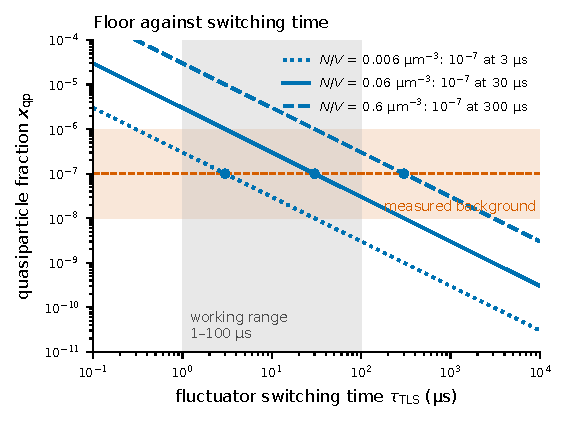
\includegraphics[width=0.62\textwidth]{figures/part3/fig_xqp_tau.pdf}
\caption{Eq.~\eqref{eq:xqp} against the fluctuator switching time for site densities $N/V=0.006$, $0.06$ and $0.6\,\mu$m$^{-3}$
($n_{\rm cp}=4\times10^6\,\mu$m$^{-3}$, $\tau_{\rm qp}=100\,\mu$s). Each line crosses the measured floor $10^{-7}$ at $\tau_{\rm TLS}=3$, 30 and
300\,$\mu$s. Grey: the 1--100\,$\mu$s working range of $\tau_{\rm TLS}$; orange band: the measured background $10^{-8}$--$10^{-6}$ \observed.
\derived\ (form) \calc\ (values)}\label{fig:xqp_tau}
\end{figure}

\section{The proposal against published observations}\label{sec:xqp_consistency}
Table~\ref{tab:xqp_obs} sets the internal-source proposal against nine published observations. The last column says what each observation does
for the proposal: whether it excludes an alternative, is consistent with the proposal, or is consistent with it and with other sources alike.
\begin{table}[htbp]\centering
\caption{The internal-source proposal against published observations.}\label{tab:xqp_obs}
\small
\begin{tabular}{p{3.2cm}p{1.4cm}p{6.2cm}p{2.6cm}}\toprule
observation & ref. & reading under the proposal & what it shows\\\midrule
excess density with an equilibrium energy distribution & \cite{Connolly2024} & a continuous source; quasiparticles relax to the gap edge far faster than $\tqp$ & consistent; any source gives it\\
same $T_1\approx80\,\mu$s above ground and deep underground & \cite{DeDominicis2026} & $T_1$ is not set by radiation-generated quasiparticles at present lifetimes & excludes radiation as the $T_1$ limit now\\
$T_1$ insensitive to shielding; tunnelling rate sensitive & \cite{Gordon2022} & much of the tunnelling is external; an internal part would remain after shielding & consistent; internal part not isolated\\
individual events uncorrelated between qubits; bursts correlated & \cite{Sundelin2026} & independent Markovian erasures at separate sites; bursts are external & consistent\\
floor follows a thermal law only above $\sim$150\,mK & \cite{Riste2013} & a non-thermal source dominates at low temperature & consistent; does not discriminate\\
TLS mostly on the junction leads & \cite{Lisenfeld2025} & the leads carry the active sites that set the erasure rate & consistent\\
TLS formed by trapped quasiparticles & \cite{deGraaf2020} & quasiparticles trapped in gap inhomogeneities add to the TLS bath (a feedback, \conjecture) & consistent\\
tunnelling depends on capacitor material and area; reduced-gap sites in some barriers & \cite{Kurter2022} & more active sites, more erasures; capacitor dependence points to external pair breaking as well & partly consistent\\
quantitative: $x_{\rm qp}\sim10^{-7}$ & \cite{Serniak2018,Diamond2022PRXQ} & Eq.~\eqref{eq:xqp} needs 60--6,000 active sites (Table~\ref{tab:xqp_sites}) & requires $N$ to be measured\\\bottomrule
\end{tabular}
\end{table}

\section{The test}\label{sec:xqp_test}
\paragraph{Prediction 1, the same-device check.} On one device, measure the five quantities $x_{\rm qp}$ (parity switching~\cite{Riste2013,Serniak2018}),
$\tau_{\rm qp}$, $\tau_{\rm TLS}$ ($1/f$ noise~\cite{Burnett2014}), the active fluctuator count $N$ (TLS spectroscopy~\cite{Lisenfeld2025}) and
the island volume $V$. Rearranging Eq.~\eqref{eq:xqp} gives the dimensionless combination the law predicts \prediction
\begin{equation}\frac{x_{\rm qp}\,n_{\rm cp}\,V\,\tau_{\rm TLS}}{N\,\tau_{\rm qp}}=2.\label{eq:xqp_invariant}\end{equation}
For $x_{\rm qp}=10^{-7}$, $n_{\rm cp}=4\times10^6\,\mu$m$^{-3}$, $V=10^4\,\mu$m$^3$, $\tau_{\rm TLS}=30\,\mu$s, $N=600$ and
$\tau_{\rm qp}=100\,\mu$s the left side is $2.000$ \calc. The right side is the pair-breaking yield; if only a fraction $p$ of events break a pair
it is $2p$. Existing data draw on different device families and measurement methods; a same-device measurement of all five quantities would be the
first direct test. Across devices, the background should scale as $N/(\tau_{\rm TLS}V)$: devices with better barriers (longer $\tau_{\rm TLS}$,
fewer active fluctuators) should show a proportionally lower floor, and better shielding should not lower it further once external sources are
gone. The proposal fails if the background does not follow $N/V$, or if it keeps falling with shielding after external sources are gone.
\paragraph{Prediction 2, the refrigerator temperature.} Below about 150\,mK the floor should not depend on $T_{\rm fridge}$ \prediction. This is
consistent with Ref.~\cite{Riste2013}; any non-thermal source predicts the same, so it is a consistency check, not a discriminating test.
\paragraph{Prediction 3, other materials.} For another superconductor, Eq.~\eqref{eq:xqp} predicts a different floor through $n_{\rm cp}=2\nu_0\Delta$,
$\tqp$, $\tTLS$ and the site density $N/V$ \prediction. The ratio of floors between two materials is
\begin{equation}\frac{x_{\rm qp,1}}{x_{\rm qp,2}}=\frac{(N/V)_1\,\tau_{\rm qp,1}\,\tau_{\rm TLS,2}\,n_{\rm cp,2}}{(N/V)_2\,\tau_{\rm qp,2}\,\tau_{\rm TLS,1}\,n_{\rm cp,1}},\label{eq:xqp_ratio}\end{equation}
each factor measurable on the devices \derived. The London depth does not enter: it sets the restoration volume of one event, not the island
density.

\section{The coherence ceiling}\label{sec:xqp_ceiling}
The quasiparticle relaxation rate of a transmon is, in the simplest estimate, $\Gamma_1^{\rm qp}=\alpha_{\rm qp}\,x_{\rm qp}\,\omega_q$ with
$\alpha_{\rm qp}\approx1$, and in full~\cite{Catelani2011PRB,Catelani2011}
\begin{equation}\Gamma_1^{\rm qp}=\frac{x_{\rm qp}}{\pi}\sqrt{\frac{2\omega_q\Delta}{\hbar}}.\label{eq:xqp_gamma1}\end{equation}
With $\Delta_{\rm Al}=182\,\mu$eV at $5$\,GHz, $x_{\rm qp}=10^{-7}$ caps $T_1$ at $0.24$\,ms (0.32\,ms in the simple estimate) and $10^{-6}$ at
$0.02$\,ms \calc. Transmons that reach $T_1\approx0.3$--$0.5$\,ms (Chapter~\ref{ch:scprimer}) carry $x_{\rm qp}\le8\times10^{-8}$ and
$\le5\times10^{-8}$; tantalum-capped niobium transmons with median $T_1$ above 0.3\,ms and maxima of 0.6\,ms~\cite{Bal2024} \observed\ require
$x_{\rm qp}\le4\times10^{-8}$ at their best \calc. At these lifetimes dielectric (TLS) loss and quasiparticles compete.

Within the proposal this part of the ceiling is endogenous \conjecture. Dielectric loss from TLS is lowered by surface treatment and external
radiation by shielding; the erasure floor is set by the cost of maintaining coherence against the TLS bath of the barrier itself. It is lowered by
changing the barrier and its fluctuators --- a barrier with longer $\tTLS$ or fewer active sites (Prediction 1) --- or a material with a larger
$n_{\rm cp}$ or a shorter $\tqp$ (Prediction 3), not by better shielding, underground operation or gap engineering alone. If the background is the
cost of holding the state, it is paid whether or not the qubit is being used.

\section{Discussion}\label{sec:xqp_discussion}
The mechanism --- a continuous Landauer maintenance cost paid at the active sites of the junction --- offers one reading of phenomena that are
usually treated separately: the persistent background $x_{\rm qp}$, the coupling between TLS and quasiparticles~\cite{deGraaf2020}, and the
equilibrium energy distribution of the excess quasiparticles~\cite{Connolly2024}. All three are consistent with the same process, the
thermodynamic cost of maintaining quantum coherence against the TLS bath at the junction \interp; the last two are also consistent with other
sources. This is a framework, not a proof. The erasure mapping and the gap-scale bath are conjectures of IAM; the London volume, the pair-breaking
yield, the diffusion over the island and the normalisation are standard superconductor physics, and they fix the form of Eq.~\eqref{eq:xqp}.
Whether the identifications describe the device is an experimental question, and the answer lies in Prediction 1: a same-device measurement of the
five quantities in Eq.~\eqref{eq:xqp_invariant} that either returns 2 or does not. No more direct test of the mechanism on existing device
platforms is known.

\section{Status}\label{sec:xqp_status}
Stands: a proposal for an internal contribution to the background quasiparticle density, from erasures at the TLS rate charged at the gap scale,
compatible with the measurements above but not established by them; the same-device test decides it \conjecture. Derived: the London
participation volume $\pi\lambda_L^3$ of one restoration (Eq.~\eqref{eq:xqp_veff}), the thermal fraction (Eq.~\eqref{eq:xqp_xth}), and, from the
proposal, the density in the field's units with quantised pair breaking and diffusion over the island (Eq.~\eqref{eq:xqp}) \derived. Predicted:
the same-device value 2 (Eq.~\eqref{eq:xqp_invariant}), the scaling with $N/(\tTLS V)$, and the material ratio (Eq.~\eqref{eq:xqp_ratio})
\prediction. Open: the active-site count $N$ for a measured device, the fluctuator switching time that governs the active sites, and whether each
erasure event breaks a pair (yield $2$) or only some do, which would lower the yield and raise the required $N$ \openprob.
